\documentclass[a4paper]{article}

\RequirePackage[12tabu, orthodox]{nag}
\usepackage[english]{babel}
\usepackage[UKenglish]{isodate}
\usepackage[parfill]{parskip}
\usepackage{float}
\usepackage{graphicx}
%\usepackage{booktabs}
\usepackage{csquotes}
\usepackage{listings}
\usepackage[margin=2.5cm]{geometry}
\usepackage{color}
\usepackage{tikz}
\usetikzlibrary{shapes.geometric, arrows}
%\usepackage[hidelinks]{hyperref}

\tikzstyle{startstop} = [rectangle, rounded corners, minimum width=3cm, minimum height=1cm,text centered, draw=black]
\tikzstyle{process} = [rectangle, minimum width=3cm, minimum height=1cm, text centered, draw=black]
\tikzstyle{decision} = [diamond, minimum width=3cm, minimum height=1cm, text centered, draw=black]
\tikzstyle{arrow} = [thick,->,>=stealth]
\tikzstyle{line} = [thick, -]

\definecolor{backcolour}{rgb}{0.95,0.95,0.92}

\lstdefinestyle{mystyle}{
	backgroundcolor=\color{backcolour},   
	basicstyle=\footnotesize,
	breakatwhitespace=false,		 
	breaklines=true,				 
	captionpos=b,					
	keepspaces=true,				 
	numbers=left,					
	numbersep=5pt,				  
	showspaces=false,				
	showstringspaces=false,
	showtabs=false,				  
	tabsize=4
}
 
\lstset{style=mystyle}

\title{COMP2121 Project - Design Manual}
\author{Kevin Zihong Ni \& Phoebe Zhou\\\small\texttt{z5025098 z1234567}}

\begin{document}

\maketitle
\tableofcontents

\section{System Flow Control} \label{sec:sfc}
\begin{center}
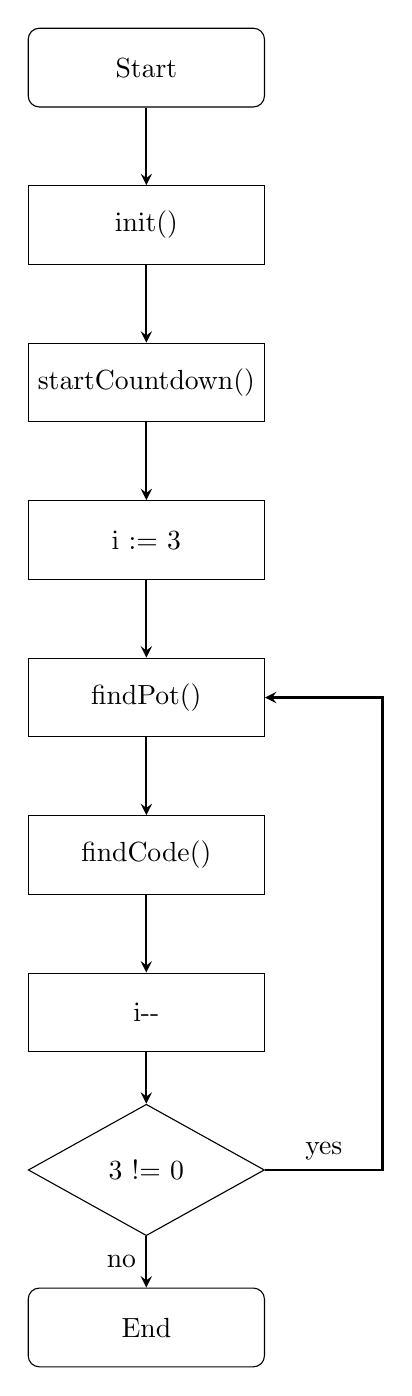
\begin{tikzpicture}[node distance=2cm]

	\node (start) [startstop] {Start};
	\node (init) [process, below of=start] {init()};
	\node (stcd) [process, below of=init] {startCountdown()};
	\node (seti) [process, below of=stcd] {i := 3};
	\node (pot) [process, below of=seti] {findPot()};
	\node (find) [process, below of=pot] {findCode()};
	\node (dec) [process, below of=find] {i-{}-};
	\node (loop) [decision, below of=dec] {3 != 0};
	\node (end) [startstop, below of=loop] {End};

	\draw [arrow] (start) -- (init);
	\draw [arrow] (init) -- (stcd);
	\draw [arrow] (stcd) -- (seti);
	\draw [arrow] (seti) -- (pot);
	\draw [arrow] (pot) -- (find);
	\draw [arrow] (find) -- (dec);
	\draw [arrow] (dec) -- (loop);
	\draw [arrow] (loop) -- node[anchor=east] {no} (end);
	\draw [arrow] (loop) -- node[anchor=south] {yes} +(3, 0) |- (pot);

\end{tikzpicture}
\end{center}

\section{Algorithm Descriptions}
At the highest level of abstraction, the algorithm of the program is very simple; it simply calls the relevant functions 
sequentially (as discussed in \ref{sec:sfc}).
The order in which the functions are called determines the screens the user must progress through in the game.


\end{document}
